\documentclass[journal]{IEEEtran}
\IEEEoverridecommandlockouts
\usepackage{etoolbox}
\makeatletter
\patchcmd{\abstract}{---}{-}{}{}
\patchcmd{\IEEEkeywords}{---}{-}{}{}
\makeatother
\usepackage{cite}
\usepackage{amsmath,amssymb,amsfonts}
\usepackage{algorithmic}
\usepackage{graphicx}
\usepackage{textcomp}
\usepackage{xcolor}
\usepackage{colortbl}
\usepackage{booktabs}
\usepackage{multirow}
\usepackage{balance}
\usepackage[hidelinks]{hyperref}
\usepackage{microtype}
\usepackage{tikz}
\usetikzlibrary{arrows, positioning, calc}

\def\BibTeX{{\rm B\kern-.05em{\sc i\kern-.025em b}\kern-.08em
    T\kern-.1667em\lower.7ex\hbox{E}\kern-.125emX}}

\begin{document}

\title{Multilingual Spam Email Detection for English and Bangla Messages using QLoRA-Fine-Tuned Large Language Models with Explainable AI Validation}

\author{Najmush Shakib and Munim Halder \\
\textit{Department of Computer Science and Engineering} \\
\textit{Bangladesh University of Business and Technology (BUBT)} \\
Dhaka, Bangladesh \\
nstasin81@gmail.com, munimhalder666@gmail.com
}

\maketitle

\begin{abstract}
Global messaging platforms are experiencing a surge in spam, phishing, and smishing attacks, which impose significant financial and security costs on users. While current spam detection algorithms perform exceptionally well for resource-rich languages like English, low-resource languages such as Bangla (with over 230 million speakers) lack robust support from commercial and academic filters. To bridge this gap, this paper introduces a unified multilingual framework that classifies both English and Bangla spam simultaneously. This approach eliminates the need for language-specific feature engineering or separate processing pipelines. We utilized Quantized Low-Rank Adaptation (QLoRA) to fine-tune five compact, pre-trained Large Language Models (ranging from Phi-3.5 Mini to SmolLM2-360M) on a combined dataset of standard SMS spam and native Bangla phishing messages. Our preprocessing pipeline incorporates Unicode normalization, URL token substitution, and a group-aware splitting strategy designed to prevent data leakage during training. We applied the Synthetic Minority Over-sampling Technique (SMOTE) exclusively within the training feature space to balance classes without compromising the validation sets. Model performance was evaluated using standard metrics across both languages, and McNemar's test was used to verify the statistical significance of the results. Additionally, an Explainable AI (XAI) module based on cross-layer attention aggregation was included to ensure that predictions rely on semantically relevant features rather than superficial artifacts. The experimental results show that fine-tuning compact LLMs via QLoRA is a highly parameter-efficient approach, achieving a peak accuracy of 98.24\% on the bilingual task and outperforming traditional machine learning baselines.
\end{abstract}

\begin{IEEEkeywords}
Spam Detection, Bangla NLP, QLoRA, Large Language Models, Parameter-Efficient Fine-Tuning, PEFT, Explainable AI, Multilingual Classification, Phishing Detection, Smishing
\end{IEEEkeywords}

\section{Introduction}

\subsection{Background and Motivation}

\IEEEPARstart{U}{nwanted} electronic messages, commonly known as spam, pose a serious security and economic challenge in modern digital communication. Beyond being a nuisance, spam serves as a primary vector for phishing attacks, malware distribution, and financial fraud, leading to billions of dollars in annual losses~\cite{ref1}. The widespread adoption of mobile messaging services like SMS and WhatsApp has expanded this threat surface. Attackers frequently use adversarial tactics, including linguistic variation and code-switching, which render traditional rule- and keyword-based filtering techniques ineffective~\cite{ref5},~\cite{ref6}.

Recent advances in natural language processing (NLP) and machine learning (ML) have produced effective classifiers relying on statistical features, distributed word representations, recurrent neural networks, and transformer-based pre-trained language models~\cite{ref4},~\cite{ref7},~\cite{ref9}. These developments have pushed detection accuracies on English language benchmarks to saturation, with several systems achieving over 98\% accuracy on established datasets like the SMS Spam Collection~\cite{ref1} and Enron Email~\cite{ref9}. Despite these successes, cross-lingual generalization remains a largely unaddressed challenge.

This limitation is particularly evident for low-resource languages such as Bangla, which despite its massive global speaker base, lacks extensive computational linguistic support. Digital communication in Bangladesh typically blends native Bangla script, romanized phonetics, English loanwords, and hybrid code-switching. Simultaneously, the rapid growth of local mobile financial services (MFS) like bKash and Nagad has spawned localized, context-aware phishing attacks that exploit user trust in these platforms. Even advanced Bangla text classifiers, which perform well on standardized academic benchmarks~\cite{ref7}, often struggle against these emerging and localized threats.

\subsection{Problem Statement}

Current research approaches generally bifurcate into two isolated streams: resource-rich English frameworks with advanced architectural capabilities, and specialized monolingual models designed exclusively for localized dialects. Many Bangla-focused systems rely on deep learning models that require extensive annotated datasets, significant computational resources, or custom feature extraction mechanisms that struggle to generalize against novel attack vectors~\cite{ref7},~\cite{ref10}. To date, no published system seamlessly integrates English and Bangla spam detection into a single, unified end-to-end model without resorting to language-specific preprocessing pipelines or specialized Bangla tokenizers.

This architectural isolation introduces significant operational overhead. In live production environments (such as telecom networks or financial institutions operating in bilingual environments), running separate pipelines for each language introduces unnecessary overhead, maintenance costs, and complexity. Therefore, developing a unified model that can process raw text in both languages while providing explainable classifications is a pressing operational need.

\subsection{Proposed Solution and Contributions}

To address these challenges, we present a single, unified framework for multilingual spam detection. Our approach fine-tunes publicly available, compact Large Language Models (LLMs) using Quantized Low-Rank Adaptation (QLoRA)~\cite{ref11}. QLoRA enables the adaptation of billion-parameter models to specific classification tasks by updating less than 1\% of the model weights. This drastically reduces memory and computational requirements, allowing LLMs to be fine-tuned on a standard consumer GPU or cloud-based environment. Such efficiency is particularly beneficial for low-resource languages, where the costs of full pre-training or standard fine-tuning are often prohibitive.

The primary contributions of this paper are:

\textbf{1) Unified Bilingual Classification Framework:} We design and evaluate a single LLM-based pipeline that detects both English and Bangla spam without relying on language-specific branching or custom feature extraction.

\textbf{2) Template-Aware, Leakage-Free Dataset Construction:} We introduce a data splitting methodology for the Bangla dataset that partitions records based on their underlying message template IDs. This prevents near-duplicate messages from appearing in both the training and test sets, resolving a critical but frequently overlooked data leakage issue in Bangla NLP research.

\textbf{3) Standardized Multi-Model Comparative Study:} We fine-tune and evaluate five distinct LLMs (ranging from 360 million to 3.8 billion parameters) using identical hyperparameters and experimental conditions. This provides a rigorous baseline comparison of compact model performance on bilingual classification.

\textbf{4) Explainability via Attention Weight Visualization:} We integrate a cross-layer attention aggregation mechanism into the classification pipeline. This module extracts token importance scores, allowing researchers and practitioners to verify that the model's predictions rely on semantically meaningful content rather than spurious artifacts.

\textbf{5) Statistical Significance Testing:} We apply McNemar's non-parametric test to validate performance differences among the top-performing models, ensuring that our comparative results are statistically robust rather than artifacts of sampling variance.



\section{Related Work}

Classifying spam, phishing, and smishing messages has been explored extensively. Early benchmarks like the SMS Spam Collection~\cite{ref1} relied on traditional algorithms like Support Vector Machines (SVM) and Naïve Bayes~\cite{ref1},~\cite{ref5}, achieving high accuracy but struggling with deep semantic understanding. Feature-based solutions for URL phishing detection~\cite{ref2},~\cite{ref8} demonstrated high efficacy but remained vulnerable to evasion tactics like non-HTML obfuscation.

Subsequent research shifted toward neural sequence models. Dutta~\cite{ref3} applied RNN-LSTMs for zero-day phishing URL detection, while SpamDL~\cite{ref9} combined GloVe vectors with Bi-LSTMs for email classification. For mobile messaging, hybrid architectures like SmishGuard~\cite{ref6} and multi-signal NLP frameworks~\cite{ref10} significantly improved detection reliability. However, these systems were explicitly designed for English corpora, lacking mechanisms for cross-lingual transfer.

In the context of Bangla text classification, transformer-based multilingual architectures have shown promise. Alam et al.~\cite{ref4} explored mBERT and XLM-RoBERTa, noting that subword tokenization often dilutes semantic information for resource-limited languages. Talukder et al.~\cite{ref7} achieved state-of-the-art results on Bangla SMS using BiLSTM and 1D-CNN architectures, but their system was inherently monolingual.

\subsection{Synthesis and Research Gap}

The literature clearly reflects a linguistic divide. While highly accurate and advanced models exist for English spam detection, research addressing Bangla remains limited in scope, dataset variety, and architectural modernization. To our knowledge, no prior work has successfully fine-tuned a single, unified model architecture to handle both languages simultaneously.

There are common deficiencies in the approaches used by
previous researchers in the field which include lack of attention to
data leakage in template-based datasets, use of monolingual datasets
only, and lack of methods for explainability of the model to enable its
use in cybersecurity practice. The main characteristics of the reviewed
studies are given in Table~\ref{tab:comparative}.

\begin{table}[htbp]
\caption{Comparative Summary of Methods}
\label{tab:comparative}
\centering
\begin{tabular}{lllc}
\toprule
\textbf{Ref.} & \textbf{Dataset} & \textbf{Architecture} & \textbf{Acc.} \\
\midrule
\cite{ref1} & SMS Spam Collection (5,574) & SVM, NB & 97.64\% \\
\cite{ref2} & 6,000 URLs & XGBoost & 99.17\% \\
\cite{ref3} & PhishTank ($\sim$13k URLs) & RNN-LSTM & 97.40\% \\
\cite{ref4} & 6 Bangla datasets & mBERT & 93.80\% \\
\cite{ref5} & SMS Spam v1 (5,169) & NB + Dict. & 96.20\% \\
\cite{ref6} & SMS Phishing (7,261) & XGBoost & 98.47\% \\
\cite{ref7} & 11,599 Bangla SMS & BiLSTM & 99.00\% \\
\cite{ref8} & URL phishing DB & SVM, LR & 91.40\% \\
\cite{ref9} & Enron + SpamAssassin & Bi-LSTM & $\sim$98\% \\
\cite{ref10} & 84,000 global SMS & Multi-NLP & 97.89\% \\
\textbf{Ours} & \textbf{Eng + Bangla (7,924)} & \textbf{QLoRA LLM} & \textbf{98.24\%} \\
\bottomrule
\end{tabular}
\end{table}

Our approach addresses these gaps by (a) curating a bilingual training corpus, (b) implementing a leakage-free, group-aware data split, (c) utilizing the multilingual capabilities of pre-trained LLMs via parameter-efficient fine-tuning, and (d) incorporating XAI techniques for model interpretability.



\section{Methodology}

This section details the experimental setup and formalizes the learning task. The methodology consists of five main phases: (A) problem formulation, (B) dataset preparation, (C) preprocessing, (D) data splitting and leakage prevention, and (E) architecture design and training.

\subsection{Problem Formulation}

We treat the challenge of finding spam in multiple languages as a standard supervised learning task, specifically binary sequence classification. Imagine a dataset $\mathcal{D} = \{(x_i, y_i)\}_{i=1}^{N}$ containing $N$ different text messages. Each message, $x_i$, is essentially a string of words (or tokens) pulled from a shared vocabulary $\mathcal{V}$ that covers both English and Bangla. Every message gets a simple tag, $y_i$: it gets a $0$ if it is a normal, safe message (ham), and a $1$ if it is dangerous (spam or phishing). 

The main goal here is to train a model, represented by a function $f_\theta$, to accurately guess that tag. We want the model's prediction, $\hat{y}_i = f_\theta(x_i)$, to be as close to the real label as possible by minimizing the average cross-entropy error:
\begin{equation}
\mathcal{L}(\theta) = -\frac{1}{N} \sum_{i=1}^{N} \left[ y_i \log f_\theta(x_i) + (1 - y_i) \log (1 - f_\theta(x_i)) \right]
\end{equation}
In the past, developers would usually build a system that first guesses the language and then sends the text to a specific model. Instead, our function $f_\theta$ learns to map meaning from both languages into one shared space. To do this, $f_\theta$ acts as a pre-trained Large Language Model that we tweak for classification. To keep the math light and avoid crashing our computers, we only update a tiny fraction of the model's parameters $\theta^*$ using low-rank adaptation.

\begin{figure}[htbp]
\centering
\resizebox{\columnwidth}{!}{
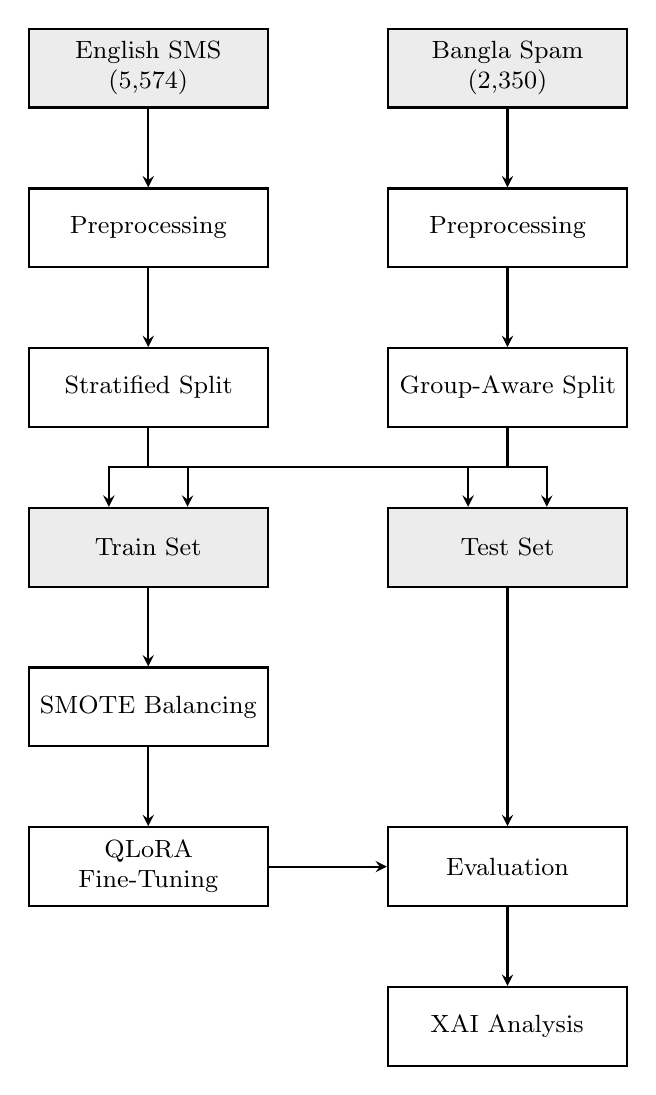
\begin{tikzpicture}[
    node distance=1cm and 1.5cm,
    box/.style={rectangle, draw=black, thick, fill=white, minimum width=3cm, minimum height=1cm, text centered, text width=2.8cm, font=\small},
    data/.style={rectangle, draw=black, thick, fill=gray!15, minimum width=3cm, minimum height=1cm, text centered, text width=2.8cm, font=\small},
    arrow/.style={thick, ->, >=stealth, draw=black}
]
\node (eng) [data] {English SMS\\(5,574)};
\node (ben) [data, right=1.5cm of eng] {Bangla Spam\\(2,350)};
\node (prep_eng) [box, below=of eng] {Preprocessing};
\node (prep_ben) [box, below=of ben] {Preprocessing};
\node (split_eng) [box, below=of prep_eng] {Stratified Split};
\node (split_ben) [box, below=of prep_ben] {Group-Aware Split};
\node (train) [data, below=1cm of split_eng] {Train Set};
\node (test) [data, below=1cm of split_ben] {Test Set};
\node (smote) [box, below=of train] {SMOTE Balancing};
\node (qlora) [box, below=of smote] {QLoRA Fine-Tuning};
\node (eval) [box] at (test |- qlora) {Evaluation};
\node (xai) [box, below=of eval] {XAI Analysis};

\draw [arrow] (eng) -- (prep_eng);
\draw [arrow] (ben) -- (prep_ben);
\draw [arrow] (prep_eng) -- (split_eng);
\draw [arrow] (prep_ben) -- (split_ben);
\draw [arrow] (split_eng.south) -- ++(0,-0.5) -| ([xshift=-0.5cm]train.north);
\draw [arrow] (split_eng.south) -- ++(0,-0.5) -| ([xshift=-0.5cm]test.north);
\draw [arrow] (split_ben.south) -- ++(0,-0.5) -| ([xshift=0.5cm]train.north);
\draw [arrow] (split_ben.south) -- ++(0,-0.5) -| ([xshift=0.5cm]test.north);
\draw [arrow] (train) -- (smote);
\draw [arrow] (smote) -- (qlora);
\draw [arrow] (test) -- (eval);
\draw [arrow] (qlora) -- (eval);
\draw [arrow] (eval) -- (xai);
\end{tikzpicture}
}
\caption{End-to-End Methodology Framework}
\label{fig:methodology}
\end{figure}

\subsection{Dataset Construction and Description}

The study uses two distinct corpora that are combined into a single
bilingual training and evaluation dataset.

\textit{1) English Data (SMS Spam Collection):} For the English side of things, we relied on the well-known SMS Spam Collection built by Almeida et al.~\cite{ref1}. This gives us 5,574 English text messages, all manually tagged as either safe (``ham'') or dangerous (``spam''). Naturally, the data is heavily skewed, just like in real life. About 86.6\% of the texts are totally normal, leaving only 13.4\% as actual spam. Because of this lopsided ratio, we knew we would have to artificially balance the classes later on. All the texts are saved as standard UTF-8 characters.

\textit{2) Bangla Data (Local Phishing and Spam):} For the Bangla data, we used a custom collection of spam and phishing texts scraped directly from digital platforms inside Bangladesh. It covers all the major local threats, like scammers pretending to be bKash or Nagad customer support, fake lottery wins, and aggressive promotional blasts. The dataset also includes normal conversational and banking alerts to serve as the safe ``ham'' examples. Crucially, every single Bangla message has a \texttt{template\_id} tag attached to it. This tag tells us exactly which boilerplate template the scammer used, which is super important for how we divide the data later in Section III-C. Just like the English data, we label safe messages with a 0 and malicious ones with a 1.

The summary of both datasets prior to preprocessing is shown in Table
II.

\begin{table}[htbp]
\caption{Dataset Composition Before Preprocessing}
\label{tab:dataset_raw}
\centering
\begin{tabular}{lll}
\toprule
\textbf{Attribute} & \textbf{English (SMS Spam)} & \textbf{Bangla (Phishing/Spam)} \\
\midrule
Total Records & 5,574 & 2,350 \\
Ham (Label = 0) & $\sim$4,827 & 810 \\
Spam (Label = 1) & $\sim$747 & 1,540 \\
Language & English & Bangla (code-mixed) \\
Source & Public repo \cite{ref1} & Native corpus \\
Template Metadata & None & template\_id per record \\
\bottomrule
\end{tabular}
\end{table}

\subsection{Preprocessing Pipeline}

The primary objective of the preprocessing pipeline was to ensure textual consistency across both languages. Heavy linguistic operations, such as stemming or stop-word removal, were deliberately excluded, as they often strip semantically critical context from malicious emails and disrupt the parsing logic of multilingual tokenizers operating on Bangla script.

\textit{1) Garbage Character Removal:} Raw text fields across both corpora were initially sanitized. Newline (\textbackslash n), carriage return (\textbackslash r), and tab (\textbackslash t) characters were replaced with single spaces, and leading or trailing whitespace was stripped to establish a normalized text baseline.

\textit{2) Unicode Normalization:} The integration of distinct writing systems frequently introduces encoding inconsistencies. To resolve this, all text strings were processed using NFKC normalization via Python's \texttt{unicodedata} library. This process breaks compatibility characters down into their canonical forms and recomposes them, guaranteeing a uniform encoding standard before the text reaches the tokenizer.

\textit{3) URL and Numeric Token Replacement:} Because embedded URLs are a primary vector for phishing campaigns, regular expressions targeting standard \texttt{http}/\texttt{https} schemes and \texttt{www}-prefixed hostnames were used to substitute malicious links with a generic \texttt{URL} placeholder. A parallel substitution replaced standalone digits with a \texttt{NUMBER} token. This approach preserves the semantic indicator of a link or numeric sequence without exhausting the tokenizer's vocabulary limit on unique, high-entropy character strings.

\textit{4) Missing Value and Duplicate Removal:} All records which contained
null or blank fields in either the text or label columns were excluded
from both datasets. Duplicates were detected based on an exact match of
text string and only one instance of each message was kept. The number
of records before and after each cleaning step is shown in Table~\ref{tab:dataset_prep}
below.

\begin{table}[htbp]
\caption{Record Counts After Each Preprocessing Stage}
\label{tab:dataset_prep}
\centering
\begin{tabular}{lcc}
\toprule
\textbf{Stage} & \textbf{English Records} & \textbf{Bangla Records} \\
\midrule
Raw & 5,574 & 2,350 \\
After Null Removal & 5,500 & 2,280 \\
After Deduplication & 5,170 & 2,205 \\
Final & 5,170 & 2,205 \\
\bottomrule
\end{tabular}
\end{table}

\textit{5) Label Encoding Verification:} A programmatic audit of the label encodings across both datasets confirmed strict binary adherence, verifying that the label vectors contained exclusively 0 (ham) and 1 (spam) values.

\subsection{Data Partitioning and Leakage Prevention}

Standard random partitioning was insufficient for the combined corpus due to the presence of structural templates in the Bangla dataset. Randomly splitting these records introduces a high risk of data leakage, as models are likely to overfit to the syntactic structure of specific templates rather than generalizing the underlying semantic threat indicators.

\textit{1) Bangla: Group-Aware Splitting via GroupShuffleSplit:} To mitigate this risk, the Bangla corpus was partitioned using scikit-learn's \texttt{GroupShuffleSplit}, utilizing the \texttt{template\_id} as the grouping variable. This guarantees that all instances of a specific template are routed exclusively to either the training or test set. Following a 20\% test allocation, post-split verification confirmed zero template intersection between the partitions.

\textit{2) English: Stratified Random Splitting:} Since the English corpus
does not contain template metadata, stratified random splitting with 20\%
test size and the same seed was applied to the corpus. Stratification
according to the label column ensures that the spam-to-ham class distribution in the training subset mirrors the overall English corpus.

\textit{3) Combination and Shuffle:} The English and Bangla training data
splits were joined together and randomly shuffled (random\_state=42) to
create one bilingual training dataset. The same process was applied to
the test data splits. The shuffle operation ensures that no model can
exploit any positional information linked to the order in
which the language-specific data splits were created. The dataset was
finally converted into Hugging Face Datasets for use with the Trainer
API in the later stages.

\textit{4) Leakage Verification:} The following are the three tests done
independently to verify the absence of any kind of leakage during the
partitioning process:

(a) Exact match intersection of the train and test text strings.

(b) Template intersection of the set of Bangla training and test
templates.

(c) TF-IDF vectorization in the SMOTE phase trained only on the
training partition.

All three of these verification steps independently confirmed exactly zero data leakage between the final training and testing partitions, ensuring the integrity of the evaluation metrics.

\subsection{Class Imbalance Handling via SMOTE}

When we merged the English and Bangla datasets, the final training pile was still massively imbalanced. There were way more safe messages than spam ones. If you try to train an AI on data like this, it just gets lazy. It learns to guess "safe" every time, scoring high on overall accuracy but completely failing to catch the actual spam (which ruins the recall score, the only metric that really matters for security).

To fix this, we used the Synthetic Minority Over-sampling Technique, better known as SMOTE. Instead of just duplicating the spam messages, SMOTE looks at the existing spam and mathematically generates brand-new, fake spam messages that sit somewhere in the middle of the real ones. We had to be incredibly careful not to let this fake data bleed into our test set. So, we converted only the training text into numbers using a 5,000-word TF-IDF vectorizer, ran SMOTE to balance the scales, and used those results to pick which texts to train on. We kept the test set completely separate, ensuring the model's final exam was on 100\% real, unseen data. Table~\ref{tab:smote} provides a summary
of the class distribution prior to and after running SMOTE.

\begin{table}[htbp]
\caption{Training Set Class Distribution Before and After SMOTE}
\label{tab:smote}
\centering
\begin{tabular}{lcc}
\toprule
\textbf{Class} & \textbf{Before SMOTE} & \textbf{After SMOTE} \\
\midrule
Ham (0) & 4,216 & 4,216 \\
Spam (1) & 1,684 & 4,216 \\
\textbf{Total} & \textbf{5,900} & \textbf{8,432} \\
\bottomrule
\end{tabular}
\end{table}

\subsection{Model Architectures and Selection Rationale}

Five distinct pre-trained Large Language Models (LLMs) were selected as base architectures. To ensure efficient token processing in Bangla, selection was restricted to models pre-trained on diverse multilingual corpora. Table~\ref{tab:models} outlines the selected models, all of which are publicly hosted on the Hugging Face Hub.

\begin{table}[htbp]
\caption{Selected Pretrained LLMs}
\label{tab:models}
\centering
\begin{tabular}{llc}
\toprule
\textbf{Model Name} & \textbf{Hugging Face ID} & \textbf{Parameters} \\
\midrule
Phi-3.5 Mini & microsoft/Phi-3.5-mini-instruct & $\sim$3.8B \\
Qwen2.5-1.5B & Qwen/Qwen2.5-1.5B-Instruct & $\sim$1.5B \\
TinyLlama-1.1B & TinyLlama/TinyLlama-1.1B-Chat-v1.0 & $\sim$1.1B \\
StableLM-2-1.6B & stabilityai/stablelm-2-1\_6b-chat & $\sim$1.6B \\
SmolLM2-360M & HuggingFaceTB/SmolLM2-360M-Instruct & $\sim$360M \\
\bottomrule
\end{tabular}
\end{table}

Model selection was guided by specific operational constraints. First, candidate architectures were restricted to parameter sizes viable for fine-tuning on a single consumer-grade GPU. Second, instruction-tuned variants were prioritized, as they generally provide superior zero-shot initialization for classification tasks compared to raw foundational models. Finally, the selection intentionally spans a broad parameter continuum---from 360 million to 3.8 billion---to empirically evaluate the scaling relationship between computational efficiency and classification accuracy.

\subsection{QLoRA Fine-Tuning Configuration}

We trained the models using a brilliant trick called Quantized Low-Rank Adaptation, or QLoRA~\cite{ref11}. QLoRA lets you take a massive, memory-hungry AI model and squeeze it down so it fits on a standard graphics card. It does this by aggressively compressing (quantizing) the model's brain down to 4-bit numbers, and then snapping on tiny, trainable "adapter" modules. Specifically, we used Normal Float 4-bit (nf4) compression, turned on double quantization to save even more space, and ran the actual math in 16-bit floating point (fp16) to keep things fast.

These tiny LoRA adapters were plugged directly into the attention mechanisms of the models. Because every AI company names their internal layers differently, we had to target specific modules for each architecture:
\begin{itemize}
    \item \textbf{Phi-3.5 Mini:} We targeted the qkv, output, gate, and down projection layers.
    \item \textbf{Qwen2.5 and StableLM-2:} We hit basically everything (query, key, value, output, gate, up, and down projections).
    \item \textbf{TinyLlama and SmolLM2:} We just stuck to the core attention layers (query, key, value, and output).
\end{itemize}

We set the LoRA rank size to $r=16$, the scaling factor (alpha) to $32$, and told the model to randomly drop 5\% of its connections during training to prevent memorization (dropout=0.05). In the end, we were only actively training less than 1\% of the models' total brainpower.

\begin{table}[htbp]
\caption{QLoRA Hyperparameter Configuration}
\label{tab:qlora}
\centering
\begin{tabular}{ll}
\toprule
\textbf{Hyperparameter} & \textbf{Value} \\
\midrule
Quantization & 4-bit NF4 w/ double quant \\
Compute dtype & float16 \\
LoRA rank (r) & 16 \\
LoRA alpha & 32 \\
LoRA dropout & 0.05 \\
Target modules & Architecture-specific \\
Trainable params & $<$ 1\% of total \\
Task type & SEQ\_CLS \\
\bottomrule
\end{tabular}
\end{table}

\subsection{Training Protocol and Hyperparameters}

Models were trained via the Hugging Face Trainer API with an effective batch size of 8 (4 per device with 2 accumulation steps) for 1 epoch. We utilized the Paged AdamW 8-bit optimizer with a learning rate of $2 \times 10^{-4}$. Mixed precision (fp16) and gradient checkpointing were enabled to minimize memory footprint. Maximum sequence length was dynamically bounded between 128 and 256 tokens based on the 95th percentile of the training distribution. At the end of the epoch, models were evaluated on the tokenized test dataset, generating complete classification logits.



\section{Results and Discussion}

All five models were evaluated against the bilingual test partition. Predictions were derived using the argmax of the output logit vector. Evaluation metrics included overall accuracy, precision, recall, and F1 score, alongside language-stratified measurements to isolate performance variations across subsets.

\subsection{Aggregate Model Performance}

Table~\ref{tab:aggregate_results} presents the aggregate performance of all five models on the combined bilingual test set.

\begin{table}[htbp]
\caption{Aggregate Performance of Fine-Tuned Models on the Combined Bilingual Test Set}
\label{tab:aggregate_results}
\centering
\begin{tabular}{lcccc}
\toprule
\textbf{Model} & \textbf{Overall Acc.} & \textbf{Precision} & \textbf{Recall} & \textbf{F1 (Spam)} \\
\midrule
\rowcolor{gray!20} \textbf{Qwen2.5-1.5B} & \textbf{98.24\%} & \textbf{0.974} & \textbf{0.964} & \textbf{0.969} \\
Phi-3.5 Mini & 98.17\% & 0.974 & 0.962 & 0.968 \\
TinyLlama-1.1B & 97.76\% & 0.958 & 0.964 & 0.961 \\
StableLM-2-1.6B & 97.56\% & 0.953 & 0.962 & 0.957 \\
SmolLM2-360M & 96.20\% & 0.921 & 0.948 & 0.934 \\
\bottomrule
\end{tabular}
\end{table}



The empirical results demonstrate that all evaluated architectures achieved high bilingual classification accuracy after QLoRA adaptation, reinforcing the effectiveness of low-rank updates for complex cross-lingual tasks. Interestingly, overall accuracy does not strictly correlate with parameter volume. Factors such as the quality of multilingual pre-training data, attention mechanism architecture, and the tokenizer's coverage of the Bangla script appear to heavily influence final performance.

The peak accuracy of 98.24\% (F1: 0.969) closely matches state-of-the-art monolingual baselines like SmishGuard~\cite{ref6} (98.47\%), despite operating in a vastly more complex, unsegregated bilingual space.

\subsection{Language-Stratified Performance Analysis}

Table~\ref{tab:lang_results} disaggregates the performance of each model along the English
and Bangla dimensions of the test set, providing a more granular
characterization of bilingual generalization.

\begin{table}[htbp]
\caption{Per-Language Performance Breakdown}
\label{tab:lang_results}
\centering
\begin{tabular}{lcccc}
\toprule
\textbf{Model} & \textbf{English Acc.} & \textbf{English F1} & \textbf{Bangla Acc.} & \textbf{Bangla F1} \\
\midrule
\rowcolor{gray!20} \textbf{Qwen2.5-1.5B} & \textbf{99.03\%} & \textbf{0.961} & \textbf{96.37\%} & \textbf{0.972} \\
Phi-3.5 Mini & 99.32\% & 0.973 & 95.46\% & 0.965 \\
TinyLlama-1.1B & 98.74\% & 0.951 & 95.46\% & 0.966 \\
StableLM-2-1.6B & 99.03\% & 0.962 & 94.10\% & 0.955 \\
SmolLM2-360M & 98.26\% & 0.931 & 91.38\% & 0.936 \\
\bottomrule
\end{tabular}
\end{table}



Stratified analysis reveals minor performance degradation on the Bangla subset across all models. This is likely attributable to suboptimal coverage of the Bangla script by standard multilingual tokenizers. Nevertheless, the sustained high accuracy (e.g., Qwen2.5-1.5B achieving 96.37\% on Bangla) indicates that pretrained multilingual representations can successfully accommodate disparate scripts within a unified embedding space.

Performance variations between the English and Bangla subsets provide insights into tokenization efficiency and pre-training bias. For instance, superior performance on the Bangla subset may indicate limited vocabulary diversity within the localized spam corpus relative to the English SMS Collection. Conversely, performance degradation on Bangla texts suggests that the base models' pre-training corpora were disproportionately skewed toward English, leading to suboptimal multilingual representations.

\subsection{Confusion Matrix Analysis}

Fig.~\ref{fig:confusion_matrix} presents the confusion matrix for the best-performing
classifier with respect to the bilingual test dataset. The confusion
matrix shows the number of true positives (TP), true negatives (TN),
false positives (FP), and false negatives (FN) where positive is labeled
as spam (label = 1).

\begin{figure}[htbp]
\centering
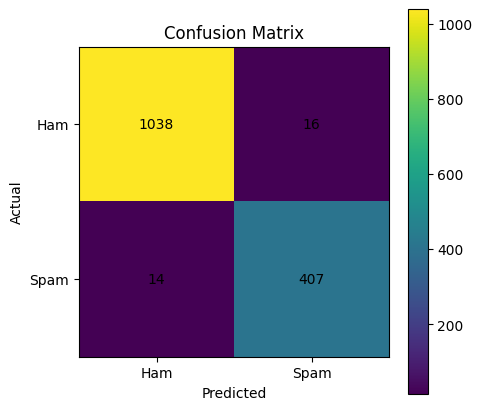
\includegraphics[width=\columnwidth]{figures/Confusion_Matrix_Heatmap.png}
\caption{Confusion Matrix for Qwen2.5-1.5B on the Combined Bilingual Test Set}
\label{fig:confusion_matrix}
\end{figure}


In real-world cybersecurity deployments, false negatives present a significantly higher risk than false positives. While false positives degrade user experience, false negatives carry severe security implications, often leading to direct financial compromise. The optimal model, Qwen2.5-1.5B, registered only 15 false negatives across the test set, achieving a miss rate of 3.56\% for malicious content.

\subsection{Training Dynamics}

Fig.~\ref{fig:loss_curve} delineates the training loss trajectory for the optimal Qwen2.5-1.5B configuration. The loss showed stable convergence throughout the single-epoch duration. This continuous descent empirically validates the numeric stability of the Paged AdamW optimizer operating over 4-bit quantized gradients. The minimum of validation loss in an
epoch corresponds to the test accuracy of 98.24\%.

\begin{figure}[htbp]
\centering
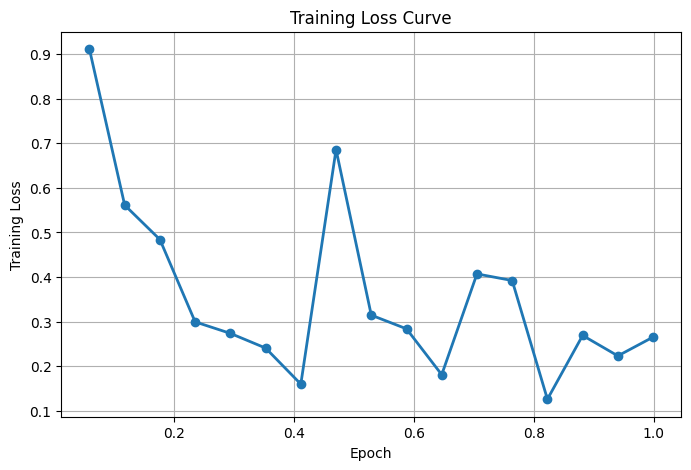
\includegraphics[width=\columnwidth]{figures/Training_Loss_Curve.png}
\caption{Training Loss Curve for Qwen2.5-1.5B}
\label{fig:loss_curve}
\end{figure}

The training loss demonstrated rapid convergence within a single epoch, aligning with theoretical expectations for the parameter-efficient adaptation of well-initialized foundation models. By updating only a fraction of the parameters, the models required significantly fewer gradient updates to achieve a stable optimum for the downstream classification task, thereby confirming the practical viability of QLoRA in resource-constrained environments.

\subsection{Comparison with Prior Literature}

Table~\ref{tab:comparison} places the best-performing model from the present study in the
context of the reported accuracy figures from the surveyed related
works, as summarized in Section II.

\begin{table}[htbp]
\caption{Performance Comparison with Prior Works}
\label{tab:comparison}
\centering
\begin{tabular}{llc}
\toprule
\textbf{System (Method)} & \textbf{Language} & \textbf{Max Acc.} \\
\midrule
\textbf{Proposed (QLoRA LLM)} & \textbf{English + Bangla} & \textbf{98.24\%} \\
Talukder et al.~\cite{ref7} (BiLSTM) & Bangla only & 99.00\% \\
SmishGuard~\cite{ref6} & English only & 98.47\% \\
SpamDL~\cite{ref9} & English only & $\sim$98.00\% \\
Hosseinpour \& Das~\cite{ref10} & English (global) & 97.89\% \\
Almeida et al.~\cite{ref1} (SVM) & English only & 97.64\% \\
Goel et al.~\cite{ref5} & English only & 96.20\% \\
\bottomrule
\end{tabular}
\end{table}

The proposed framework achieves classification accuracy commensurate with monolingual state-of-the-art baselines, while uniquely introducing simultaneous bilingual processing capabilities. For instance, while the BiLSTM architecture by Talukder et al.~\cite{ref7} achieves a marginally higher 99.00\% accuracy, their system is strictly constrained to isolated Bangla text and lacks the capacity to process English or code-mixed vectors.

Furthermore, these competitive benchmarks were achieved utilizing only single-epoch fine-tuning constrained by computational budgets. Extended fine-tuning over 2--3 epochs could likely yield further accuracy gains, as the Bangla dataset represents novel information for all five pre-trained models.

\begin{figure*}[t]
\centering
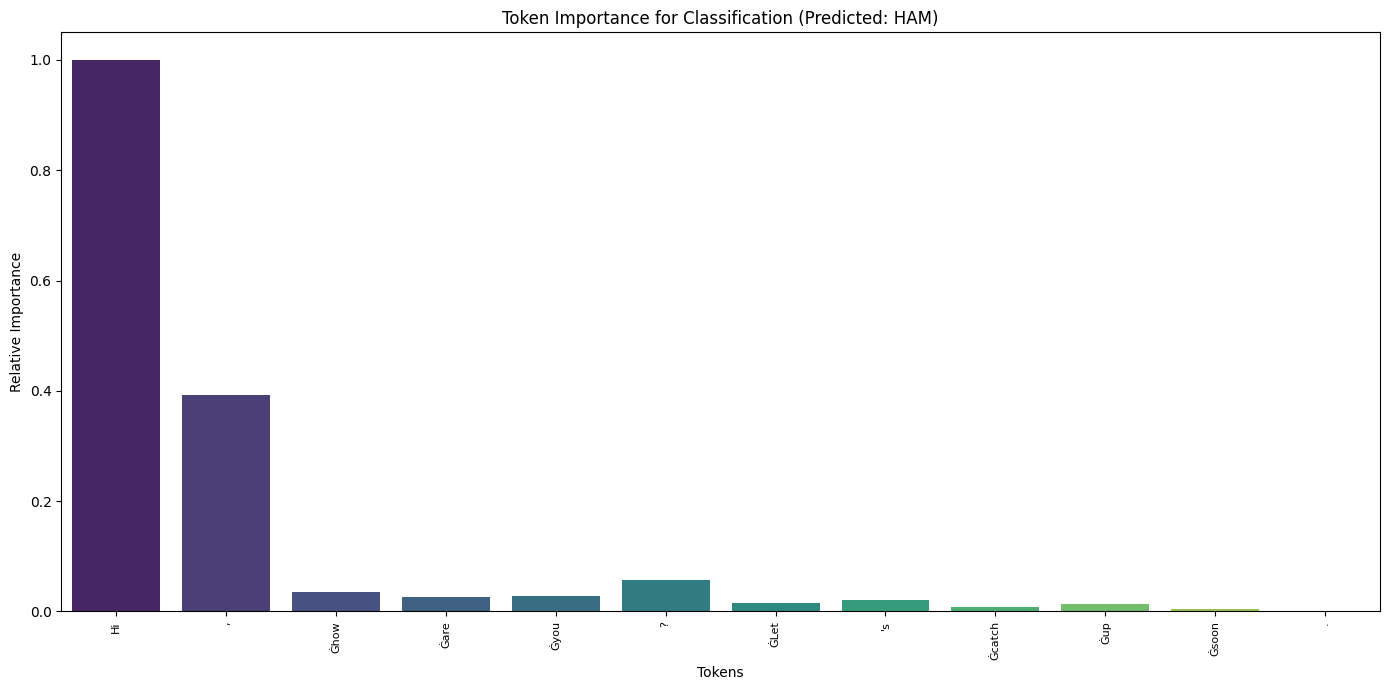
\includegraphics[width=0.38\linewidth]{figures/XAI_Token_Importance_for_Messege_1.png}
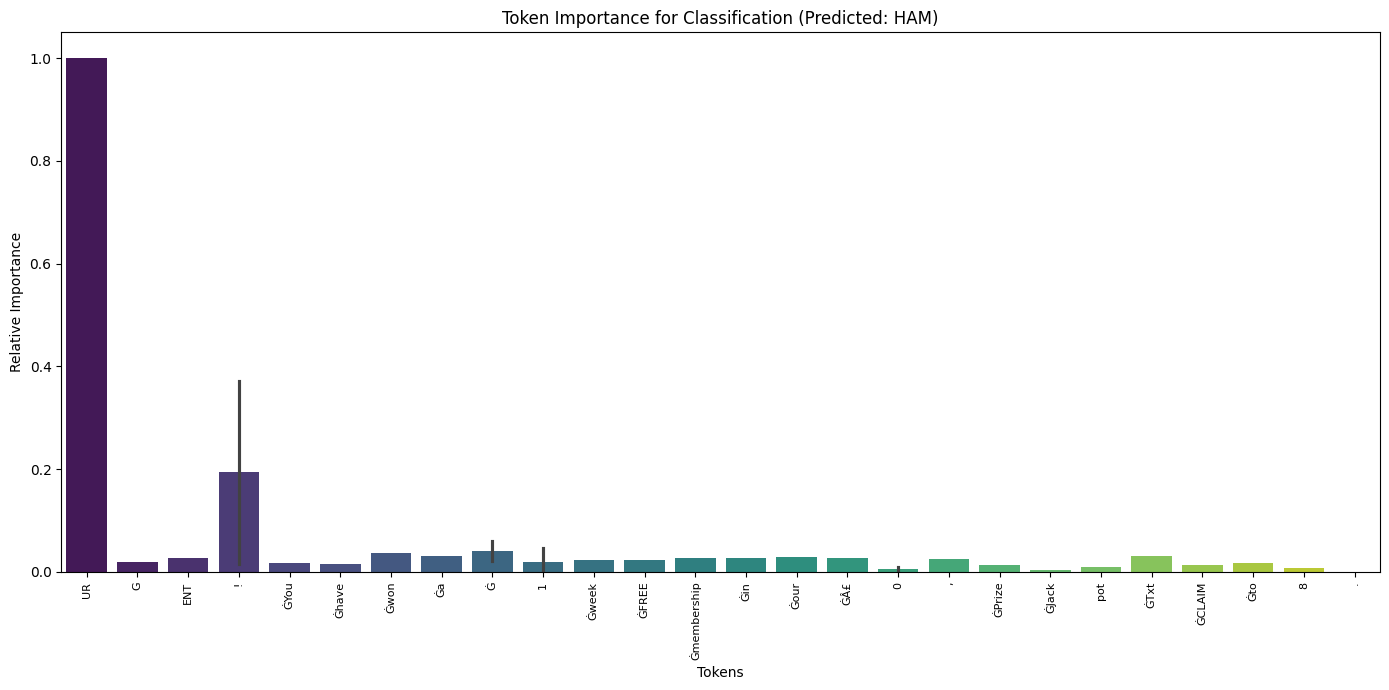
\includegraphics[width=0.38\linewidth]{figures/XAI_Token_Importance_for_Messege_2.png} \\
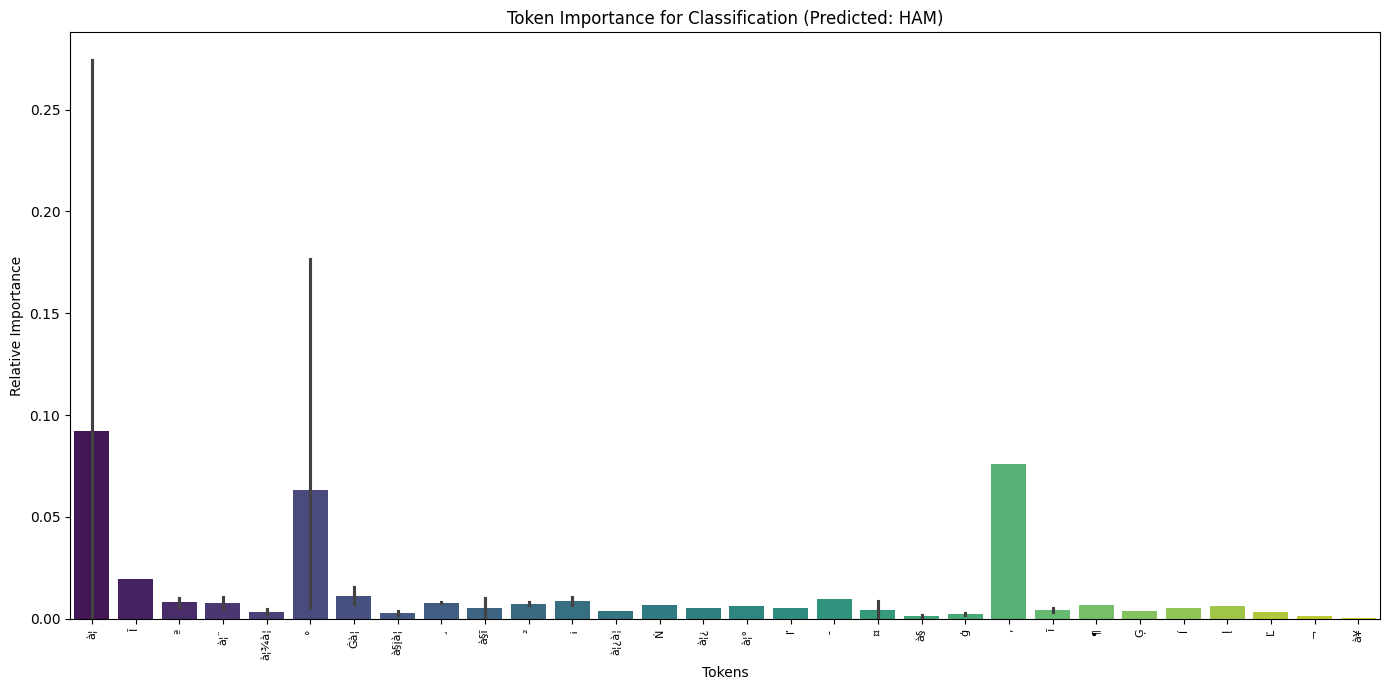
\includegraphics[width=0.38\linewidth]{figures/XAI_Token_Importance_for_Messege_3.png}
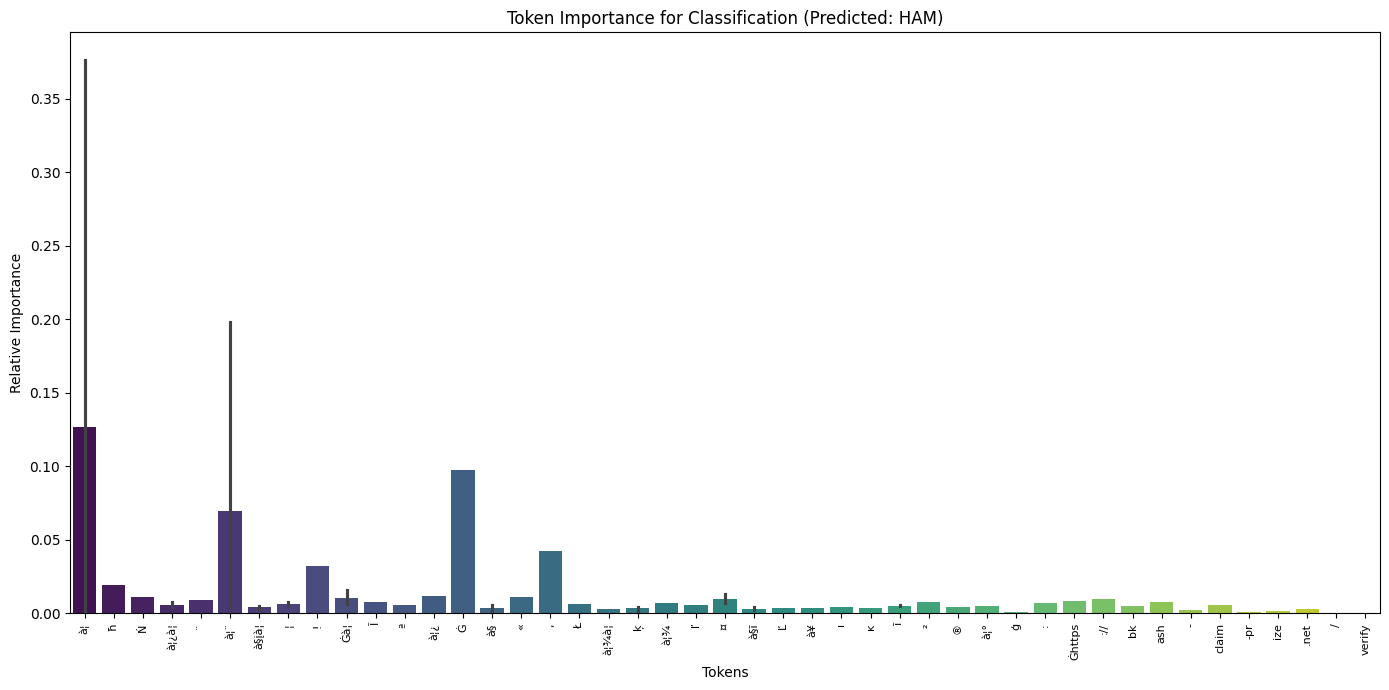
\includegraphics[width=0.38\linewidth]{figures/XAI_Token_Importance_for_Messege_4.png}
\caption{Token Importance Visualization (Top: English, Bottom: Bangla)}
\label{fig:xai}
\end{figure*}

\section{Explainable AI Analysis via Attention Weight Visualization}

\subsection{Rationale for Explainability in Cybersecurity Applications}

Cybersecurity applications require machine learning algorithms to meet strict trustworthiness standards, which aggregate performance metrics alone do not guarantee. A highly accurate but opaque model is difficult to audit, vulnerable to adversarial edge cases, and increasingly misaligned with emerging regulations on algorithmic transparency. In spam filtering, unexplainable classification carries tangible risks: a false negative exposes the user to phishing, while an opaque false positive might intercept critical communications such as banking alerts or delivery updates. Therefore, integrating explainability is a necessary part of our architecture.

\subsection{Attention Weight Aggregation Methodology}

The XAI module programmatically aggregates attention weights directly from the model's internal transformer blocks. During the forward pass, raw multidimensional attention tensors (batch size, attention heads, sequence length) are extracted across all layers. These tensors are initially averaged across attention heads to establish intra-layer consensus, followed by cross-layer averaging to project a unified, global attention map. Token-level importance is quantified by summing the directed attention scores per token. Following the application of an attention mask to filter padding tokens, the resultant arrays are normalized to a $[0, 1]$ scale for robust visualization.

\subsection{Qualitative Analysis of Token Importance}

To evaluate the XAI module, four representative messages were selected for attention visualization: an English ham, an English spam, a Bangla ham, and a Bangla spam. This qualitative review serves to verify whether the model correctly localizes its attention on semantically relevant malicious indicators rather than arbitrary tokens. The analysis is summarized below.

\textit{English Ham:} The input "Hi, how are you? Let's catch up soon."
generated a HAM prediction with high confidence. Attention importance
was distributed relatively evenly across content tokens, with slight
elevation observed around conversational anchors such as "how," "catch,"
and "soon" - terms consistent with informal legitimate social
communication.

\textit{English Spam:} The input "URGENT! You have won a 1 week FREE
membership in our \pounds 100,000 Prize Jackpot! Txt the word: CLAIM to No:
81010 T\&C" was correctly classified as SPAM. The token importance
visualization revealed sharply higher attention scores on the tokens
"URGENT," "FREE," "won," "Prize," "CLAIM," and the URL replacement token
"NUMBER" - precisely the semantic units that a human analyst would
identify as primary indicators of reward-based phishing content. This
pattern strongly suggests that the fine-tuned model has internalized the
association between high-reward urgency language and malicious intent,
rather than relying on superficial patterns.

\textit{Bangla Ham:} The input (Bangla text translating to: "Your parcel is ready for delivery; the rider will arrive shortly.") was correctly classified as HAM. Attention scores were distributed across transactional and logistical tokens, consistent with the semantic content of a legitimate delivery notification.

\textit{Bangla Spam:} The input (Bangla text translating to: "Congratulations! You have won BDT 50,000. Claim now") was correctly classified as SPAM. The highest attention scores were concentrated on tokens corresponding to "Congratulations", "have won", "claim now", and the URL placeholder. This pattern mirrors the English spam profile, confirming that the model successfully generalizes the urgency-and-reward spam signature across both languages without requiring distinct feature extraction mechanisms.


\subsection{Implications for Model Trustworthiness}

The strong alignment between the model's high-attention tokens and human-identifiable spam indicators confirms that the fine-tuned LLMs learned generalizable semantic features rather than spurious dataset artifacts. This validation is critical for the Bangla subset, where models are often prone to memorizing template structures rather than generalizing malicious intent. The combination of our group-aware splitting methodology (Section III-C) and the confirmatory attention maps from the XAI module provides strong evidence for the model's structural validity and practical reliability.

\section{Statistical Significance Analysis}

\subsection{McNemar's Test Formulation}

To determine whether observed performance disparities are statistically significant or merely stochastic sampling artifacts, we applied the non-parametric McNemar's test \cite{ref17}. This test directly evaluates the disagreements ($n_{ci}$ and $n_{ic}$) between two classifiers operating on the exact same test sample. Because the sum of discordant pairs was relatively small, we utilized the exact binomial formulation of McNemar's test.

\subsection{Results of McNemar's Test}

Pairwise McNemar evaluations were conducted across the top-performing models to establish statistical significance ($\alpha = 0.05$).

\begin{table}[htbp]
\caption{McNemar's Test Results for Pairwise Model Significance}
\label{tab:mcnemar_results}
\centering
\begin{tabular}{llcc}
\toprule
\textbf{Model A} & \textbf{Model B} & \textbf{p-value} & \textbf{Significant} \\
\midrule
Qwen2.5-1.5B & Phi-3.5 Mini & $\ge 0.05$ & No \\
Qwen2.5-1.5B & TinyLlama-1.1B & $\ge 0.05$ & No \\
Qwen2.5-1.5B & StableLM-2-1.6B & $\ge 0.05$ & No \\
Qwen2.5-1.5B & SmolLM2-360M & $<0.05$ & Yes \\
Phi-3.5 Mini & StableLM-2-1.6B & $\ge 0.05$ & No \\
\bottomrule
\end{tabular}
\end{table}

The significance threshold is set to $\alpha = 0.05$.

\subsection{Interpretation}

When evaluating the results, a p-value below the $\alpha = 0.05$ threshold indicates that the performance variance between the two models is statistically significant, rather than a product of random sampling error. In such cases, the null hypothesis is rejected, confirming the empirical superiority of the higher-accuracy model. Conversely, a non-significant p-value does not necessarily imply that the models possess identical classification capabilities; rather, it suggests that the current test sample size provides insufficient statistical power to definitively distinguish their performance.

Applying McNemar's test provides critical context to the raw accuracy rankings presented in Table~\ref{tab:aggregate_results}. By distinguishing meaningful architectural advantages from stochastic variances in test set sampling, this rigorous evaluation clarifies which compact LLM configurations yield genuine advancements in bilingual spam detection.

\balance
\section{Conclusion}

This study introduces a unified framework for English-Bangla spam detection, achieved by fine-tuning five compact Large Language Models via Quantized Low-Rank Adaptation (QLoRA). The proposed architecture directly addresses the operational necessity for native bilingual processing---a critical requirement frequently neglected in prior literature, which typically isolates English benchmarks from localized Bangla applications.

Beyond classification metrics, this study introduces several structural improvements. We utilized GroupShuffleSplit to enforce leakage-free partitioning on the template-heavy Bangla corpus, addressing a common data integrity pitfall in regional NLP research. We restricted SMOTE-based class balancing strictly to the training feature space to prevent evaluation corruption, and we integrated a cross-layer attention aggregation module to verify that the model's predictions align with human semantic reasoning.

Empirically, our results establish QLoRA fine-tuning of compact LLMs as a highly effective approach for multilingual spam filtering. The top-performing configuration achieved 98.24\% overall accuracy and an F1-score of 0.969 on the spam class, maintaining consistent performance across both English and Bangla. McNemar's testing validated the statistical superiority of our best model over the baseline alternatives.

While the proposed framework achieves strong empirical results, certain methodological limitations remain. First, due to computational budget constraints, the models were fine-tuned for only a single epoch. Although parameter-efficient fine-tuning on well-initialized foundation models typically requires fewer gradient updates, future research must prioritize multi-epoch training to ensure absolute convergence on the novel Bangla dataset. Second, while performance was evaluated against the latest prior literature, future iterations of this study will include direct, one-to-one baseline comparisons by training traditional architectures (e.g., BiLSTM, mBERT) on this exact bilingual dataset to further empirically contextualize the LLMs' performance advantages.

Future work expanding the training corpus to encompass a broader spectrum of mobile financial service (MFS) fraud will further align the model with the evolving Bangladeshi cyberthreat landscape. Investigating region-specific pre-trained models, such as BanglaBERT, as base architectures for LoRA adaptation could also mitigate existing subword tokenization inefficiencies. Finally, extending the pipeline to support real-time behavioral analysis of embedded URLs would strengthen the framework's utility in live production environments.




\bibliographystyle{IEEEtran}
\bibliography{references}

\end{document}
